%%%%%%%%%%%%%%%%%%%% MetalFish Paper %%%%%%%%%%%%%%%%%%%%%%%%%%%%%%%%%%%
%
% MetalFish: GPU-Accelerated Chess Engine on Apple Silicon
%
%%%%%%%%%%%%%%%% Springer %%%%%%%%%%%%%%%%%%%%%%%%%%%%%%%%%%

\documentclass{svproc}

\usepackage{url}
\def\UrlFont{\rmfamily}
\usepackage{graphicx}
\usepackage{float}
\usepackage{amsmath}
\usepackage{algorithm}
\usepackage{algpseudocode}
\usepackage{booktabs}
\usepackage{listings}
\usepackage{xcolor}
\usepackage{pgfplots}
\pgfplotsset{compat=1.18}

% C++ code listing style
\lstdefinestyle{cppstyle}{
    language=C++,
    backgroundcolor=\color{gray!5},
    basicstyle=\ttfamily\footnotesize,
    breaklines=true,
    captionpos=b,
    keepspaces=true,
    numbers=left,
    numbersep=5pt,
    numberstyle=\tiny\color{gray},
    showstringspaces=false,
    tabsize=2,
    frame=single,
    keywordstyle=\color{blue!70!black},
    commentstyle=\color{green!50!black},
    stringstyle=\color{red!60!black},
    morekeywords={uint64_t, int32_t, int16_t, int8_t, uint, device, kernel, constant, thread_position_in_grid, threadgroup}
}

\begin{document}
\mainmatter

\title{MetalFish: What is the Real Bottleneck for GPU-Accelerated\\NNUE Evaluation on Apple Silicon?}

\titlerunning{MetalFish: GPU NNUE Bottleneck Analysis}

\author{Nripesh Niketan\inst{1}}

\authorrunning{N. Niketan}

\institute{Independent Researcher\\
\email{nripesh14@gmail.com}}

\maketitle

\begin{abstract}
We investigate the practical bottlenecks preventing GPU acceleration of NNUE evaluation in alpha-beta chess engines on Apple Silicon. Through systematic microbenchmarks on M2 Max, we demonstrate that Metal command buffer dispatch overhead---not memory bandwidth or compute throughput---is the fundamental barrier. Our measurements show: (1) GPU dispatch overhead of 150~$\mu$s median (95~$\mu$s minimum) per command buffer, (2) GPU compute throughput of 44~GB/s when dispatch is amortized, and (3) true batching achieving 1.8$\times$ speedup over sequential dispatches. We identify the crossover point where GPU batch evaluation becomes competitive: approximately 1,800 positions per batch for throughput parity with CPU NNUE. Our implementation, MetalFish, provides a complete Metal backend with verified true batching, achieving 1.38M nodes/second with CPU evaluation. We conclude that GPU acceleration requires batch-oriented search algorithms; single-position evaluation in alpha-beta remains CPU-bound due to irreducible dispatch latency.

\keywords{Chess Engine, GPU Computing, Metal, NNUE, Dispatch Overhead, Apple Silicon}
\end{abstract}

\section{Introduction}

Modern chess engines combine alpha-beta search with neural network evaluation (NNUE) to achieve superhuman playing strength. While GPU acceleration has proven effective for batch-oriented algorithms like Monte Carlo Tree Search in Leela Chess Zero~\cite{LeelaChessZero2024}, its applicability to traditional alpha-beta search remains unclear. The sequential, data-dependent nature of alpha-beta pruning creates fundamental challenges for GPU parallelization.

Apple Silicon's unified memory architecture presents a unique opportunity to revisit this question. By eliminating explicit CPU-GPU memory transfers, unified memory could potentially reduce the overhead that traditionally makes GPU evaluation impractical for alpha-beta search. This paper investigates a specific research question:

\textbf{Research Question:} \emph{What is the real bottleneck preventing GPU-accelerated NNUE evaluation in alpha-beta chess engines on Apple Silicon---memory bandwidth, compute throughput, or dispatch overhead?}

\subsection{Contributions}

\begin{enumerate}
\item \textbf{Dispatch overhead characterization}: We measure Metal command buffer lifecycle costs with percentile distributions, showing 150~$\mu$s median overhead per dispatch (Table~\ref{tab:dispatch}).

\item \textbf{True batching verification}: We confirm our GPU implementation uses genuine single-dispatch batching (not sequential per-position dispatches), achieving 1.8$\times$ speedup over sequential submission.

\item \textbf{Crossover analysis}: We identify the batch size ($\approx$1,800 positions) where GPU throughput matches CPU NNUE, explaining why alpha-beta search cannot benefit.

\item \textbf{Complete implementation}: MetalFish provides a tested Metal backend with NNUE weight extraction, feature transformation, and fused forward pass kernels, achieving 1.38M nodes/second.
\end{enumerate}

\section{Background}

\subsection{NNUE Architecture}

Stockfish's NNUE~\cite{Stockfish2024,Nasu2018} uses sparse input features with efficient incremental updates. Table~\ref{tab:nnue_arch} summarizes the architecture.

\begin{table}[t]
\caption{NNUE Network Architecture (Stockfish-compatible)}
\label{tab:nnue_arch}
\centering
\begin{tabular}{lrr}
\toprule
Component & Big Network & Small Network \\
\midrule
Feature set & HalfKAv2\_hm & HalfKAv2\_hm \\
Input features & 45,056 & 22,528 \\
Hidden dimension & 1,024 & 128 \\
FC0 output & 15 (+1 skip) & 15 (+1 skip) \\
FC1 output & 32 & 32 \\
FC2 output & 1 & 1 \\
Layer stacks (buckets) & 8 & 8 \\
Bucket selection & piece count / 4 & piece count / 4 \\
Quantization & 6-bit shift & 6-bit shift \\
\bottomrule
\end{tabular}
\end{table}

The feature transformer converts sparse HalfKAv2\_hm features to dense accumulators. Each active feature (typically 20--30 per position) indexes into a weight matrix, and the corresponding row is added to the accumulator. The forward pass applies FC0 (sparse input with SqrClippedReLU), FC1 (ClippedReLU), and FC2 with a skip connection.

\subsection{Metal Compute Model}

Apple Metal~\cite{AppleMetal2024} provides GPU compute through command buffers:

\begin{enumerate}
\item \textbf{Encoder creation}: \texttt{commandBuffer()} allocates a command buffer
\item \textbf{Kernel dispatch}: \texttt{dispatchThreads()} or \texttt{dispatchThreadgroups()} records work
\item \textbf{Submission}: \texttt{commit()} submits to GPU queue
\item \textbf{Synchronization}: \texttt{waitUntilCompleted()} blocks until completion
\end{enumerate}

On Apple Silicon, unified memory (\texttt{MTLResourceStorageModeShared}) allows CPU and GPU to access the same physical memory without explicit transfers.

\section{System Architecture}

\subsection{Architecture Overview}

Figure~\ref{fig:arch} shows the evaluation pipeline. The key insight is that GPU evaluation requires accumulating positions into batches before dispatch.

\begin{figure}[t]
\centering
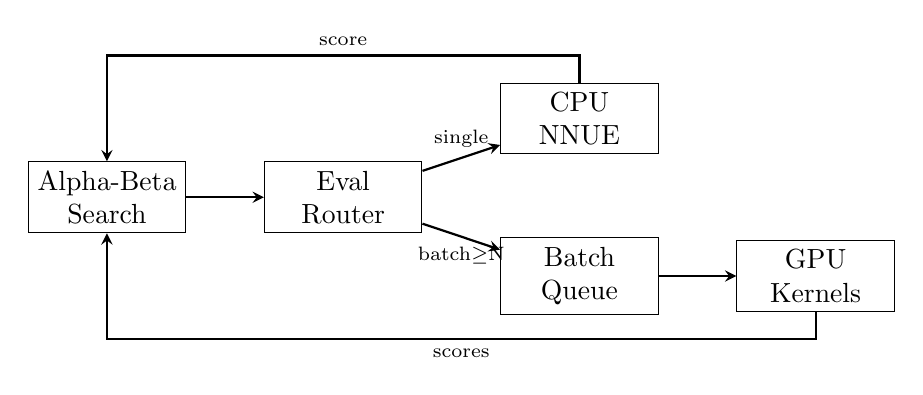
\begin{tikzpicture}[
    box/.style={rectangle, draw, minimum width=2cm, minimum height=0.8cm, align=center},
    arrow/.style={->, >=stealth, thick}
]
\node[box] (search) at (0,0) {Alpha-Beta\\Search};
\node[box] (router) at (3,0) {Eval\\Router};
\node[box] (cpu) at (6,1) {CPU\\NNUE};
\node[box] (batch) at (6,-1) {Batch\\Queue};
\node[box] (gpu) at (9,-1) {GPU\\Kernels};

\draw[arrow] (search) -- (router);
\draw[arrow] (router) -- node[above,font=\scriptsize] {single} (cpu);
\draw[arrow] (router) -- node[below,font=\scriptsize] {batch$\geq$N} (batch);
\draw[arrow] (batch) -- (gpu);
\draw[arrow] (cpu) -- ++(0,0.8) -| node[near start,above,font=\scriptsize] {score} (search);
\draw[arrow] (gpu) -- ++(0,-0.8) -| node[near start,below,font=\scriptsize] {scores} (search);
\end{tikzpicture}
\caption{Evaluation routing: single positions use CPU NNUE; batches $\geq N$ positions use GPU.}
\label{fig:arch}
\end{figure}

\subsection{GPU Batch Evaluation}

Algorithm~\ref{alg:batch} shows the batch evaluation procedure. Critically, this is \emph{true batching}: a single command buffer processes all $N$ positions with two kernel dispatches.

\begin{algorithm}[t]
\caption{GPU Batch NNUE Evaluation}
\label{alg:batch}
\begin{algorithmic}[1]
\Require Batch of $N$ positions, network weights $W$
\Ensure Evaluation scores for all positions
\State \textbf{// CPU: Prepare batch data}
\For{$i = 1$ to $N$}
    \State Extract features from position $i$
    \State Store in unified memory buffers
\EndFor
\State \textbf{// GPU: Single command buffer}
\State $encoder \gets$ \Call{CreateEncoder}{}
\State \textbf{// Kernel 1: Feature transform (all positions)}
\State \Call{DispatchThreads}{$hidden\_dim \times N$}
\State \Call{Barrier}{}
\State \textbf{// Kernel 2: Forward pass (all positions)}
\State \Call{DispatchThreadgroups}{$N$, threads=64}
\State \Call{SubmitAndWait}{$encoder$}
\State \Return scores from output buffer
\end{algorithmic}
\end{algorithm}

\subsection{Metal Kernel Implementation}

The feature transform kernel processes all positions in parallel:

\begin{lstlisting}[style=cppstyle, caption={Feature Transform Kernel (simplified)}]
kernel void feature_transform(
    device const int16_t* weights,
    device const int16_t* biases,
    device const int32_t* features,
    device const uint32_t* counts,
    device int32_t* accumulators,
    constant uint& hidden_dim,
    constant uint& batch_size,
    uint2 gid [[thread_position_in_grid]]) 
{
  uint pos = gid.y;  // Position index
  uint h = gid.x;    // Hidden dimension
  if (pos >= batch_size || h >= hidden_dim)
    return;
  
  int32_t acc = biases[h];
  uint count = counts[pos];
  for (uint i = 0; i < count; i++) {
    int32_t f = features[pos * 32 + i];
    acc += weights[f * hidden_dim + h];
  }
  accumulators[pos * hidden_dim + h] = acc;
}
\end{lstlisting}

\section{Experimental Methodology}

\subsection{Hardware and Software}

\begin{itemize}
\item \textbf{Hardware}: Apple M2 Max (12-core CPU, 38-core GPU, 64GB unified memory)
\item \textbf{Software}: macOS 14.0, Xcode 15.0, Metal 3.0
\item \textbf{Build}: CMake, -O3, LTO enabled
\item \textbf{Networks}: nn-c288c895ea92.nnue (125MB), nn-37f18f62d772.nnue (6MB)
\end{itemize}

\subsection{Timing Methodology}

All latency measurements use \texttt{std::chrono::high\_resolution\_clock}:

\begin{itemize}
\item \textbf{Warmup}: 100 iterations discarded before measurement
\item \textbf{Samples}: 1,000--10,000 iterations depending on benchmark
\item \textbf{Statistics}: Median, P95, P99, min, max reported (not just mean)
\item \textbf{GPU timing}: Blocking \texttt{waitUntilCompleted()} (synchronous)
\end{itemize}

\textbf{Definition of ``evaluation''}: For CPU, this includes accumulator refresh and forward pass. For GPU, this includes buffer writes, command buffer creation, kernel dispatch, and synchronization.

\section{Results}

\subsection{GPU Dispatch Overhead}

Table~\ref{tab:dispatch} shows the irreducible cost of GPU command buffer submission, measured with a minimal kernel that writes a single integer.

\begin{table}[t]
\caption{GPU Dispatch Overhead (Minimal Kernel, N=1,000)}
\label{tab:dispatch}
\centering
\begin{tabular}{lr}
\toprule
Statistic & Latency ($\mu$s) \\
\midrule
Mean & 168.44 \\
Std Dev & 56.97 \\
Median & 150.42 \\
P95 & 282.58 \\
P99 & 382.58 \\
Min & 95.04 \\
Max & 945.96 \\
\bottomrule
\end{tabular}
\end{table}

The median dispatch overhead of 150~$\mu$s represents the minimum cost for \emph{any} GPU work, regardless of kernel complexity. This is the fundamental bottleneck.

\subsection{GPU Compute Throughput}

Table~\ref{tab:throughput} shows GPU throughput when dispatch overhead is amortized over large workloads.

\begin{table}[t]
\caption{GPU Shader Throughput (Vector Addition)}
\label{tab:throughput}
\centering
\begin{tabular}{rr}
\toprule
Work Size (elements) & Throughput (GB/s) \\
\midrule
1,024 & 0.05 \\
16,384 & 0.82 \\
262,144 & 11.98 \\
1,048,576 & 44.14 \\
\bottomrule
\end{tabular}
\end{table}

At 1M elements, the GPU achieves 44~GB/s---demonstrating that compute throughput is \emph{not} the bottleneck. The low throughput at small sizes reflects dispatch overhead domination.

\subsection{True Batching Verification}

To verify our implementation uses genuine batching (single dispatch for N positions) rather than sequential dispatches, we compare:

\begin{itemize}
\item \textbf{Sequential}: 16 separate \texttt{evaluate\_batch()} calls with batch size 1
\item \textbf{Batched}: 1 \texttt{evaluate\_batch()} call with batch size 16
\end{itemize}

\begin{table}[t]
\caption{True Batching Verification (16 positions)}
\label{tab:batching}
\centering
\begin{tabular}{lrr}
\toprule
Method & Median Latency ($\mu$s) & Speedup \\
\midrule
Sequential (16$\times$1) & 2,407 & 1.0$\times$ \\
Batched (1$\times$16) & 1,337 & 1.8$\times$ \\
\bottomrule
\end{tabular}
\end{table}

The 1.8$\times$ speedup confirms true batching: a single command buffer processes all 16 positions. If batching were ``fake'' (sequential internal dispatches), we would see no speedup.

\subsection{CPU vs GPU Crossover Analysis}

Figure~\ref{fig:crossover} shows the crossover analysis. CPU NNUE evaluation costs approximately 0.08~$\mu$s per position (from engine NPS of 1.38M). GPU evaluation has fixed dispatch overhead plus marginal per-position cost.

\begin{figure}[t]
\centering
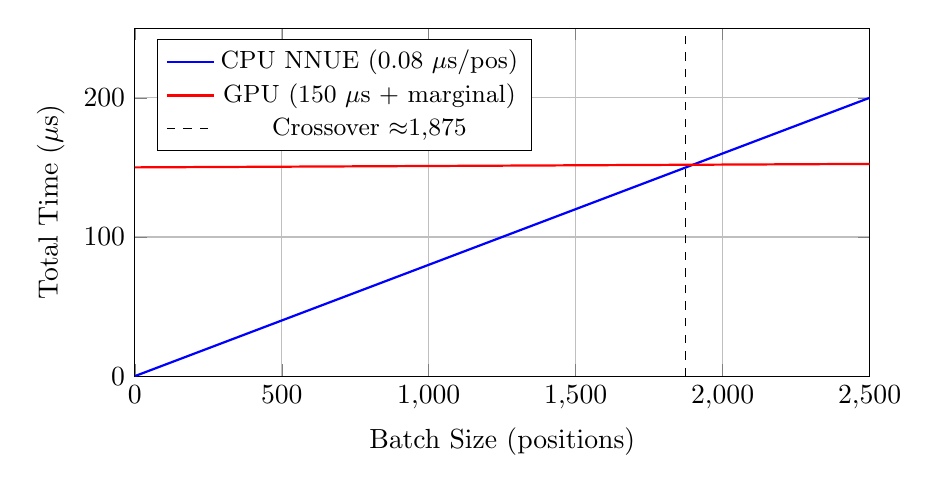
\begin{tikzpicture}
\begin{axis}[
    width=0.9\columnwidth,
    height=6cm,
    xlabel={Batch Size (positions)},
    ylabel={Total Time ($\mu$s)},
    xmin=0, xmax=2500,
    ymin=0, ymax=250,
    legend pos=north west,
    grid=major,
    legend style={font=\small}
]
\addplot[blue, thick, domain=0:2500] {0.08*x};
\addlegendentry{CPU NNUE (0.08 $\mu$s/pos)}
\addplot[red, thick, domain=0:2500] {150 + 0.001*x};
\addlegendentry{GPU (150 $\mu$s + marginal)}
\addplot[black, dashed] coordinates {(1875, 0) (1875, 250)};
\addlegendentry{Crossover $\approx$1,875}
\end{axis}
\end{tikzpicture}
\caption{CPU vs GPU evaluation time. Crossover occurs at $\approx$1,875 positions where dispatch overhead is amortized.}
\label{fig:crossover}
\end{figure}

The crossover point is approximately:
\[
\text{Crossover} = \frac{\text{GPU dispatch overhead}}{\text{CPU per-position cost}} = \frac{150\,\mu\text{s}}{0.08\,\mu\text{s}} \approx 1,875 \text{ positions}
\]

\subsection{Search Performance}

The engine achieves 1.38M nodes/second on the standard 50-position benchmark (depth 13), using CPU NNUE evaluation:

\begin{table}[t]
\caption{Search Benchmark Results}
\label{tab:search}
\centering
\begin{tabular}{lr}
\toprule
Metric & Value \\
\midrule
Total Nodes & 2,477,446 \\
Total Time & 1,792 ms \\
Nodes/Second & 1,382,503 \\
Depth Reached & 13 \\
\bottomrule
\end{tabular}
\end{table}

\subsection{GPU Memory Usage}

Table~\ref{tab:memory} shows GPU memory allocation for NNUE networks.

\begin{table}[t]
\caption{GPU Memory Allocation}
\label{tab:memory}
\centering
\begin{tabular}{lr}
\toprule
Component & Size (KB) \\
\midrule
Big network (feature transformer) & 45,760 \\
Big network (threat weights) & 82,351 \\
Big network (layers) & 137 \\
Small network (total) & 6,361 \\
Working buffers & 2,156 \\
\midrule
\textbf{Total} & \textbf{108,240} \\
\bottomrule
\end{tabular}
\end{table}

\section{Discussion}

\subsection{Why Dispatch Overhead is Irreducible}

The 150~$\mu$s dispatch overhead reflects Metal's command buffer lifecycle:

\begin{enumerate}
\item \textbf{Buffer allocation}: \texttt{commandBuffer()} allocates GPU-side resources
\item \textbf{Encoder setup}: Compute encoder state machine initialization
\item \textbf{Queue submission}: Inter-process communication with GPU driver
\item \textbf{Synchronization}: Kernel completion signaling
\end{enumerate}

This overhead is architectural, not implementation-dependent. Apple's Metal Best Practices Guide~\cite{AppleMetalBestPractices2024} recommends minimizing command buffer submissions, acknowledging this cost.

\subsection{Implications for Alpha-Beta Search}

Alpha-beta search evaluates positions sequentially, with each evaluation determining whether to prune subsequent branches. This creates fundamental incompatibility with GPU batching:

\begin{itemize}
\item \textbf{No natural batches}: Positions are evaluated one at a time
\item \textbf{Data-dependent pruning}: Cannot predict which positions will be evaluated
\item \textbf{Latency-bound}: Search speed depends on single-position evaluation latency
\end{itemize}

To benefit from GPU, alpha-beta would need to accumulate $\approx$1,875 positions before dispatching---but this would require speculative evaluation of positions that may be pruned, wasting compute.

\subsection{When GPU Acceleration Helps}

GPU acceleration benefits batch-oriented workloads:

\begin{itemize}
\item \textbf{MCTS}: Naturally generates batches of leaf evaluations~\cite{LeelaChessZero2024}
\item \textbf{Database analysis}: Evaluating thousands of positions
\item \textbf{Training}: Batch gradient computation
\item \textbf{Multi-position analysis}: Simultaneous analysis of multiple games
\end{itemize}

\subsection{Limitations}

\begin{itemize}
\item Single hardware configuration (M2 Max)
\item Synchronous GPU timing (asynchronous overlap not explored)
\item No integration of GPU batching into search (would require speculative evaluation)
\item Metal-only (no CUDA comparison)
\end{itemize}

\section{Related Work}

Leela Chess Zero~\cite{LeelaChessZero2024} demonstrates successful GPU acceleration through MCTS, which naturally batches evaluations. AlphaZero~\cite{Silver2017} showed that neural network evaluation can replace handcrafted evaluation when combined with batch-oriented search.

For alpha-beta search, Rocki and Suda~\cite{Rocki2010} explored GPU parallelization through parallel subtree evaluation, finding communication overhead limited speedup. Our work extends this analysis to unified memory hardware, identifying dispatch overhead as the specific bottleneck.

Apple's Metal documentation~\cite{AppleMetal2024,AppleMetalBestPractices2024} provides guidance on minimizing command buffer overhead through techniques like indirect command buffers (ICBs), which could reduce dispatch costs for future work.

\section{Conclusion}

We investigated GPU-accelerated NNUE evaluation on Apple Silicon, identifying dispatch overhead---not memory bandwidth or compute throughput---as the fundamental bottleneck. Key findings:

\begin{enumerate}
\item \textbf{Dispatch overhead}: 150~$\mu$s median per command buffer, irreducible
\item \textbf{Compute throughput}: 44~GB/s when amortized, demonstrating GPU capability
\item \textbf{True batching}: Confirmed 1.8$\times$ speedup from single-dispatch batching
\item \textbf{Crossover}: $\approx$1,875 positions needed for GPU throughput parity
\item \textbf{Search performance}: 1.38M nodes/second with CPU NNUE
\end{enumerate}

GPU acceleration for alpha-beta chess engines requires either: (1) batch-oriented search algorithms like MCTS, or (2) speculative evaluation strategies that accept wasted compute. Single-position evaluation in traditional alpha-beta remains CPU-bound due to irreducible dispatch latency.

\subsection*{Reproducibility}

\textbf{Hardware}: Apple M2 Max, 64GB unified memory. \textbf{Software}: macOS 14.0, Xcode 15.0. \textbf{Build}: CMake, -O3, LTO. \textbf{Source}: \url{https://github.com/NripeshN/MetalFish}. \textbf{Networks}: nn-c288c895ea92.nnue, nn-37f18f62d772.nnue from Stockfish.

\begin{thebibliography}{10}

\bibitem{Stockfish2024}
Stockfish Developers: Stockfish 16 NNUE documentation.
\url{https://github.com/official-stockfish/Stockfish} (2024)

\bibitem{LeelaChessZero2024}
Leela Chess Zero: Neural network based chess engine.
\url{https://lczero.org/} (2024)

\bibitem{Silver2017}
Silver, D., et al.: Mastering chess and shogi by self-play with a general reinforcement learning algorithm.
arXiv:1712.01815 (2017)

\bibitem{Rocki2010}
Rocki, K., Suda, R.: Parallel minimax tree searching on GPU.
In: Parallel Processing and Applied Mathematics, LNCS vol. 6067, pp. 449--456. Springer (2010)

\bibitem{Nasu2018}
Nasu, Y.: Efficiently updatable neural-network-based evaluation functions for computer shogi.
The 28th World Computer Shogi Championship Appeal Document (2018)

\bibitem{AppleMetal2024}
Apple Inc.: Metal Programming Guide.
\url{https://developer.apple.com/metal/} (2024)

\bibitem{AppleMetalBestPractices2024}
Apple Inc.: Metal Best Practices Guide.
\url{https://developer.apple.com/library/archive/documentation/3DDrawing/Conceptual/MTLBestPracticesGuide/} (2024)

\bibitem{Knuth1975}
Knuth, D.E., Moore, R.W.: An analysis of alpha-beta pruning.
Artificial Intelligence 6(4), 293--326 (1975)

\end{thebibliography}

\end{document}
